\section{Geodetics}

During the implementation of the design during this sprint, geodetic considerations became necessary. Geodetics is the science of measurement and representation of the Earth~\cite{website:Wikipedia-geodesy}. In normal day to day work we consider Euclidean distances on the surface of the Earth to be straight lines. While this is usually good enough, it will not remain as simple when the distances start to scale up, or the requirements for accuracy increase. Therefore we must consider the shape of the Earth.

Depending on the required level of precision, the Earth can be modelled as a sphere or as an oblate spheroid\sinote{insert reference}\cite{}. Both are, however, still only approximations, as the actual shape of the Earth is more complex when considering differences in the Earth's surface, such as elevation and tectonic movement.

If a sphere or an oblate spheroid is accepted as a good approximation, we still need to consider that we are working with non-euclidean geometry.

This section will try to outline the considerations on these matters which were done during the sprint, and how they affected the project.

\subsection{Spatial Referencing of the Earth}

Latitude/longitude is a geographical coordinate system, which can be used to reference positions on the surface of the Earth. Latitude ranges 180 degrees in total, with the Equator being 0 degrees and the North and South poles being 90 degrees\sinote{insert reference}\cite{}. Longitude ranges 360 degrees in total, with the prime meridian being 0 degrees and the antipodes being 180 degrees west or east\sinote{insert reference}\cite{}. Different prime meridians can be used, but for this project the International Reference Meridian will be used\sinote{insert reference}\cite{}. It should be noted that latitude is a finite range, whereas longitude is a cyclic range which allows distances to cross directly from 180 degrees west to 180 degrees east. This can be troublesome as the distance between two points can be ambiguous. Take for an example the distance from 179 degrees west to 179 degrees east. Depending on the direction the distance can either be 2 degrees or 358 degrees, or if we denote western degrees as negative, we can potentially get the nonsensical distance of minus 2 degrees. In this sprint we will not make any effort into automatically handling this, since we will not do any calculations near the edges, however, since it could potentially result in logical bugs, it should be handled eventually.

In this report we use the WGS84 standard for spatial referencing. It was created and is maintained by the United States Department of Defense \cite{WGS84} and is used in the GPS system. In the WGS84 system, latitude and longitude is not noted by their direction, but instead ranges from -90 to 90 and from -180 to 180 respectively.

\subsection{Calculating Distances}

Due to the nature of non-euclidean geometry, special formulae should be used when calculating geometry on the surface of the Earth. A good example of this is the Pythagorean theorem $a^2 + b^2 = c^2$. If the triangle is curved around a sphere, it becomes necessary to modify the formula to $cos(\frac{a}{R}) \cdot cos(\frac{b}{R}) = cos(\frac{c}{R})$ where $R$ is the radius of the sphere\cite{website:lawofcosines}.

\begin{figure}[htbp]
    \centering
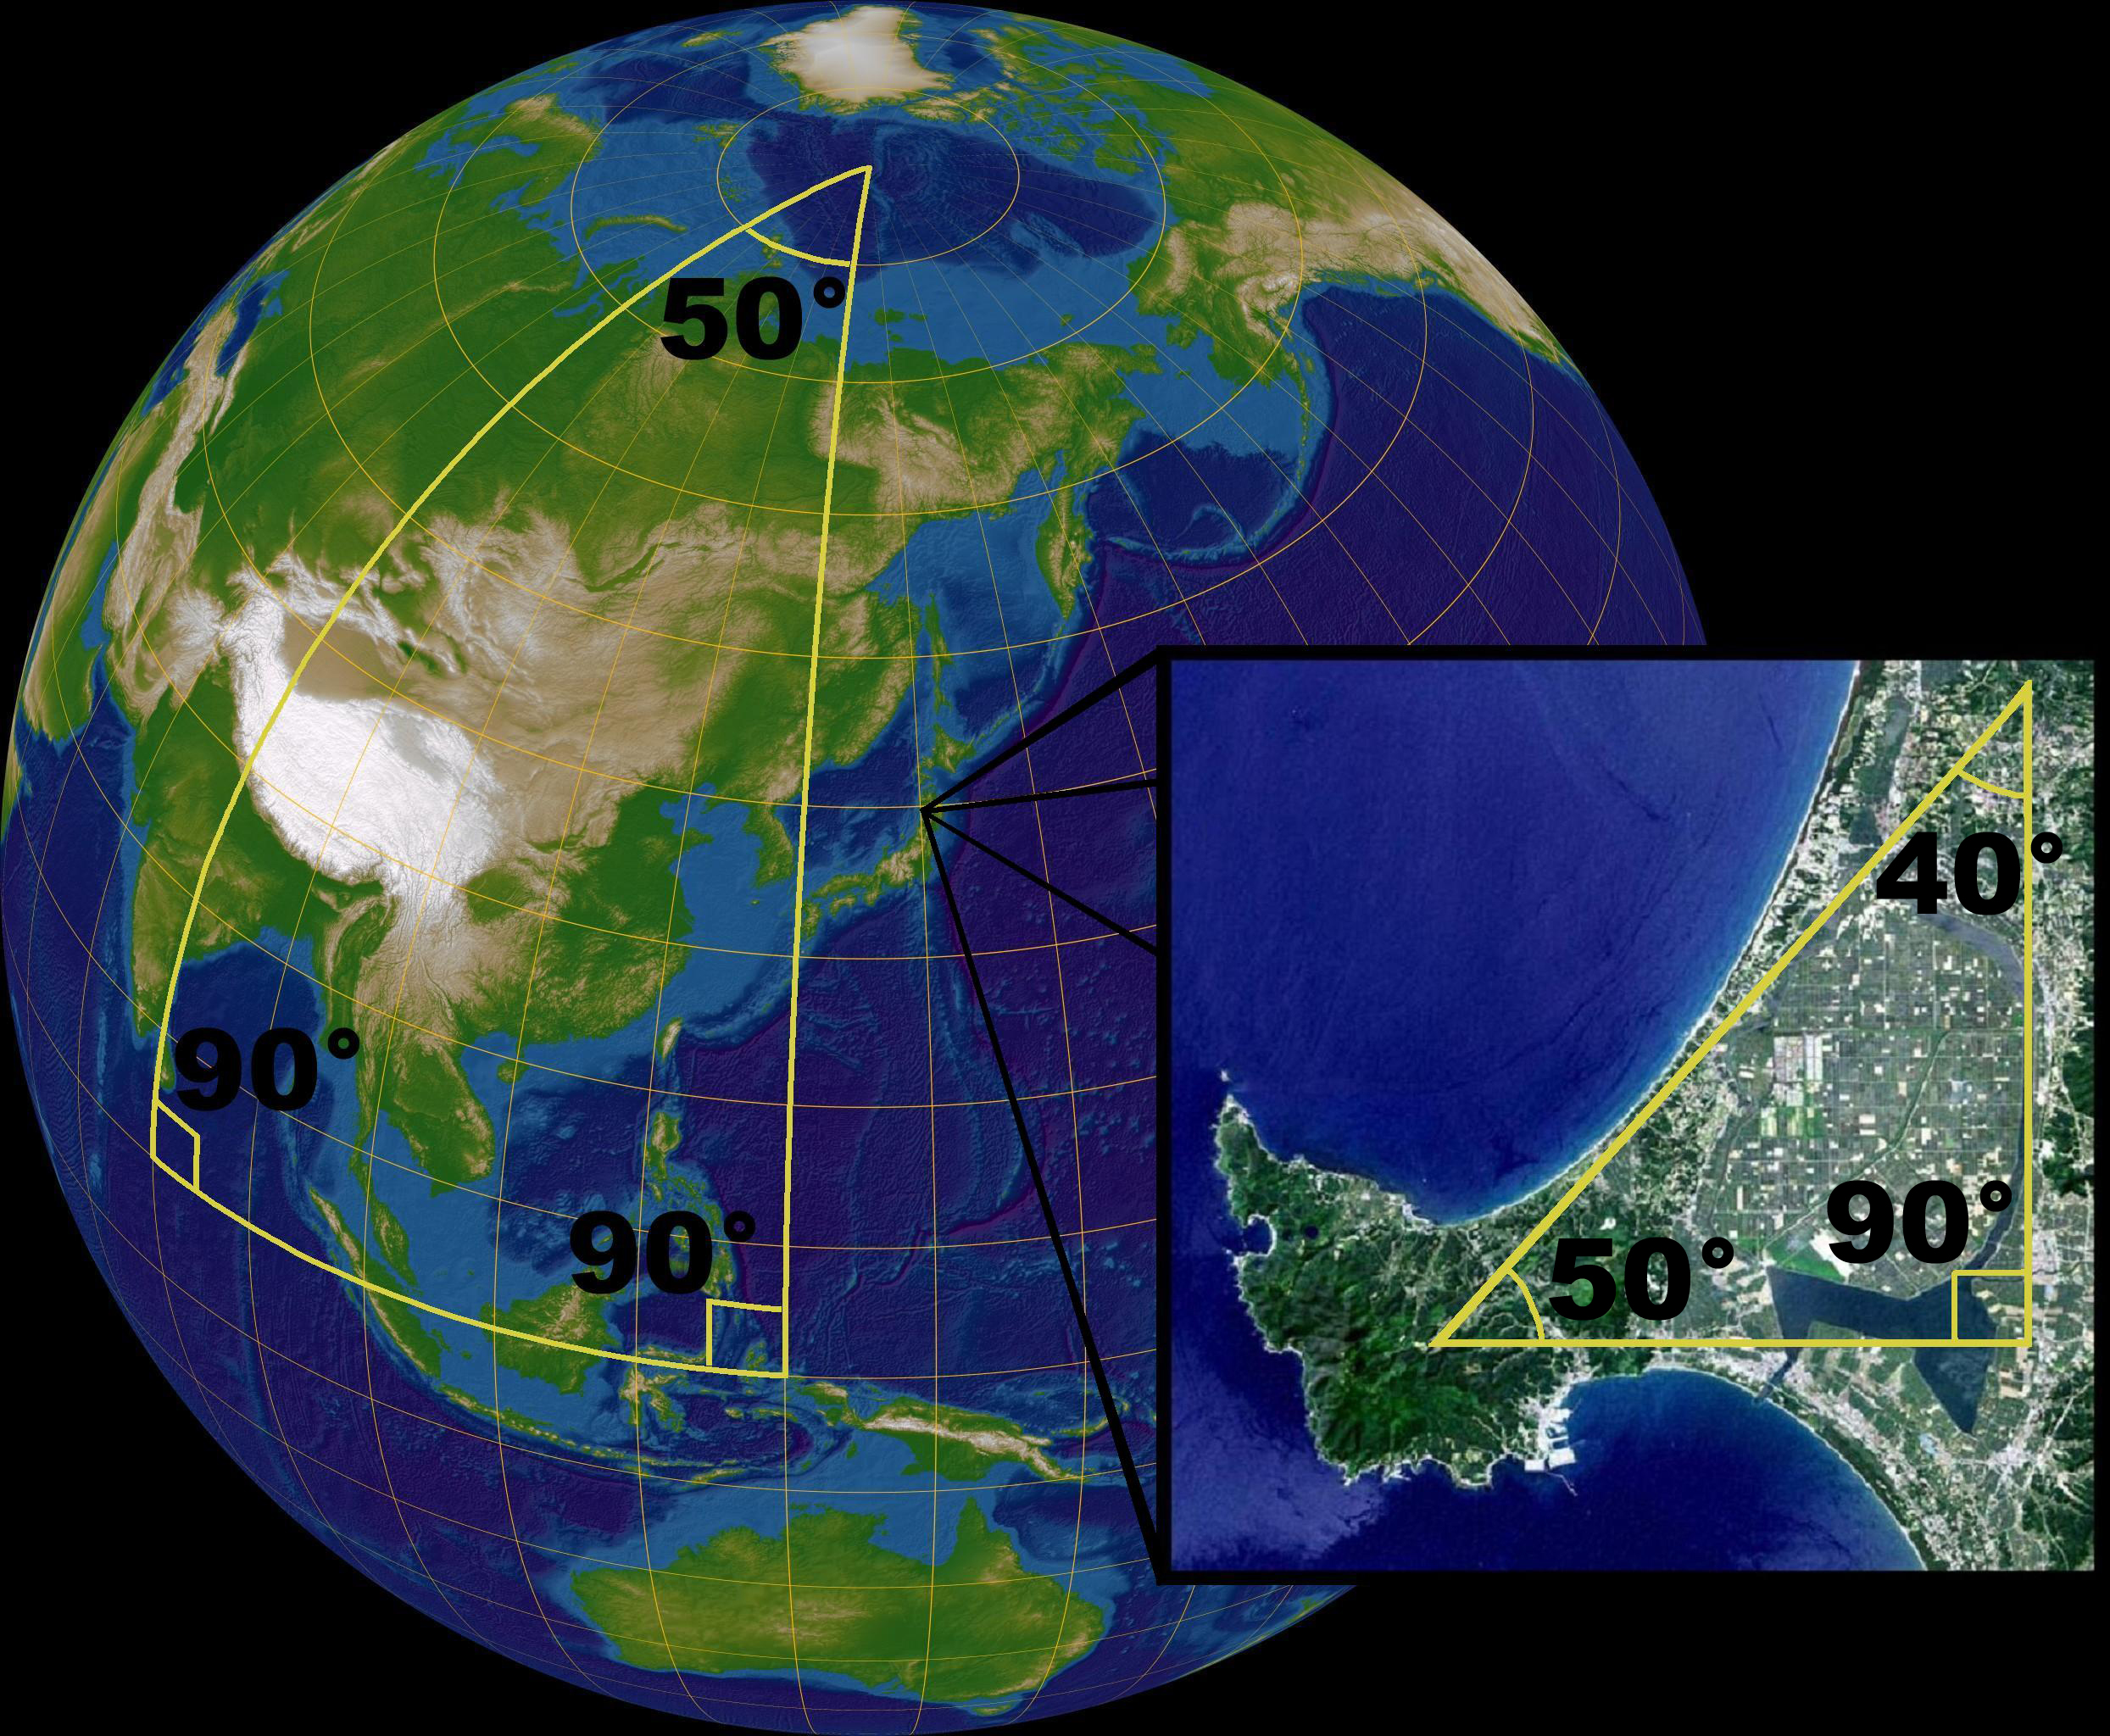
\includegraphics[width=\textwidth/2]{noneuclidean.jpg}
\caption[Triangle on sphere]{Triangle on sphere showing properties of Non-euclidean geometry~\cite{earthtriangle}.}
\label{noneuclidean}
\end{figure}

As a consequence of this, calculating absolute distances between two positions on Earth becomes a bit more complicated. There are two different methods worth considering for solving the problem, the Haversine formula and Vincenty's formulae.

Vincenty's formulae~\cite{vincenty} is an iterative method for calculating the distance between two points on an oblate spheroid with a high accuracy. However this accuracy can come at the cost of potentially thousands of iterations.

The Haversine formula considers a simplified Earth in the shape of a sphere, and can be derived from the spherical law of cosines~\cite{website:lawofcosines}. It lacks in accuracy in comparison with Vincenty's method but it is not as costly a calculation.

Whenever distances are calculated, we should consider the required properties and evaluate which method is more appropriate. However for this project we will be using Haversine since the limited distances will minimize the inaccuracies of the formula, and that the better performance is helpful during the calculation of the crowd conditions described in \cref{sec:related_work}.


\subsection{Projection}

Whenever a two dimensional map of the Earth is made, it will be subjected to distortion~\cite{projectionalbum}. However the level and area of distortion will differ depending on the choice of map projection. Some projections will distort the poles but have accurate information near the Equator, while others might try to distort the oceans and keep landmasses accurate~\cite{website:Wikipedia-mapprojections}.

The projection used in this project is the Web Mercator projection~\cite{webmercator}, which is based on the WGS84 standard presented earlier. The projection is a faster version of the Mercator projection, since it assumes a spherical Earth instead of an ellipsoidal Earth. It was popularised by Google Maps and is used by many web-based services. The projection is conformal, meaning that it preserves angles locally, making it good for navigation, however it lacks in the ability to accurately represent area~\cite{mercatorcritique}. In \cref{tissots} we can see the distortion illustrated with tissot's indicatrices~\cite{tissot}. This kind of illustration projects multiple circles of the same actual dimensions on a map, in order to show how the map distorts the surface of the Earth.

\begin{figure}[htbp]
    \centering
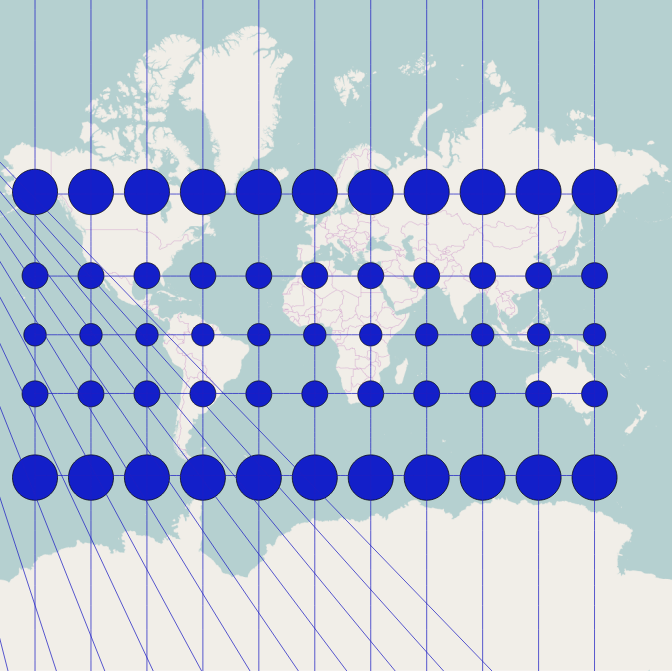
\includegraphics[width=\textwidth/2]{tissotmercator.png}
\caption{Tissot's indicatrices on Web Mercator projection.}
\label{tissots}
\end{figure}

We can see how the northern and southern circles are distorted in area, but does not stretch into ellipses, which illustrate the property that the map projects distances from east to west with the same level of distortion as distances from south to north. We can also see that the lines of longitudes and latitudes remain straight and parallel, which also displays the conformal property of the projection. The projection is unable to display the two poles, since the distortion would stretch infinitely as we approach them.

Since the solution will not require distant area comparison, and primarily need to display a given local area in relation to itself, this projection suits the project well.


\subsection{Summary}

In summary, the development of the application should involve considerations on geodetics in order to sustain precision. Referencing of positions on the Earth is done relative to the Earth according to the WGS84 standard, and as such any geometric calculation must consider the consequences of the shape of the Earth. This will mainly manifest itself in the use of the Haversine formula and derivations thereof. Projection will be done using the Web Mercator standard, which will allow for a direct translation between projection and referencing. These choices aim to minimise the geodetic problems, allowing for a more clean implementation.




































































